\documentclass[a4paper,11pt]{article}

\usepackage[utf8]{inputenc}    % Pour que LaTeX comprenne les accents.
\usepackage{times}             % Police de caractères
\usepackage[english]{babel}     % Traitement du texte adapté aux règles typographiques
                               % de la langue donnée en option (e.g., pour l'espacement
                               % après les ponctuations
\usepackage[T1]{fontenc}
\usepackage{amsmath, amsthm, amssymb} 
\usepackage{dsfont}  % pour les indicatrices 
\usepackage{graphicx}                               
\sloppy              % Ne pas faire déborder les lignes dans la marge


\newtheorem{lemma}{Lemma}
\newtheorem{cons}{Consequences}

\theoremstyle{definition}
\newtheorem{definition}{Definition}
\newtheorem{process}{Process}

\theoremstyle{remark}
\newtheorem{remark}{Remark}

\title{Throwing needles on a colored plane.}

\begin{document}
\maketitle

\begin{abstract} the same in english \end{abstract}

(The computations for the lower bound, using parallel stripes, are the same.)

\section{Definitions}


For the intuitive idea of ``throwing a needle uniformly on the plane'' to make sense in a probabilistic approach, we choose to make the following assumption : 
the colouring of the plane is \textit{periodic} - that is, there is a basis of two vectors, $u$ and $v$, such that translations along these vectors leave the colouring unchanged. Thereafter, we denote $\mathcal{P}$ the parallelogram defined by these vectors. And we consider needle throwing processes on this parallelogram.

\begin{definition}
A graph $(V,E) $ is said to be a \emph{unit distance graph}, if it has a representation in the plane, with all edges having length $1$.
\end{definition}


\begin{process}
Formally, consider the following random variables :
\begin{itemize}
  \item let $A_1$ (the lowest point of the needle) be a point chosen uniformly in $\mathcal{P}$ ;
  \item let $\theta$ be an independent angle chosen uniformly in $[0;\pi[$ ;
  \item let $A_2$ (the highest point of the needle) be $A_1 + e^{i \theta}$.
\end{itemize}
\end{process}

Note that $A_2$ may be outside of $\mathcal{P}$. In that case, $c(A_2)$ is defined using the periodicity of the colouring.
Our goal is to evaluate and minimize the probability that both ends have the same color.

\begin{remark}
Note that there are several couples of vectors $(u,v)$ forming an appropriate basis for the 
colouring. Nonetheless, we can prove that the probabilities does not depend on this choice. 
\end{remark}


We consider the following process : \\
\begin{process}
Given a unit distance graph $(G,V)$, label all the edges with numbers from $1$ to $|E|$. Choose : 
\begin{itemize}
\item one point $A_0$ uniformly on the initial parallelogram $\mathcal{P}$ for the origin of the graph.
\item an angle $\theta$ uniformly in $[0;2\pi[$, to rotate the graph
\item and an index $i$ in $[|1;|E||]$.
\end{itemize}
Then, rotate the graph by the angle $\theta$, translate it so that the origin falls on  $A_0$, and take the needle corresponding to the position of $i^{th}$ edge of the graph obtained. 
\end{process}
\vspace{1 cm} 

\section{Process equivalence}
\begin{lemma}\label{huitre}
Let $(A,B)$ denote the needle obtained by the original process, and
$(A',B')$ the one obtained by the second process. Let $c_1$ and $c_2$ denote two colors, and $c$, the application giving the color of a point. Then, we have :\\
 $$\mathbb{P}(c(A) = c_1 , c(B) = c_2) = \mathbb{P}(c(A') = c_1, c(B') = c_2) $$ \\
 \\
 In particular, this means that the probability doesn't depend on the graph chosen. For a graph with only two vertices, we exactly get the initial process.
\end{lemma}

\begin{proof}
Conventions : 
\begin{itemize}
\item we take a graph $G=(V,E)$, and $m = |E|$, the number of edges.

\item as usual, $\mathcal{P}$ is the parallelogram obtained by the periodicity of the colouring.

\item $\mathcal{A(P)}$ is the area of the parallelogram we are considering.

\item $i$ is the index of one of the edges of $G$.

\item we denote $z_i$ the complex coordinates of one vertex of the $i^{th}$ edge.

\item $\theta_i$ denotes the angle made by the $i^{th}$ edge of the graph. The complex coordinates of the vertices of the $i^{th}$ edges before rotation/translation are then $z_i $ and $z_i + e^{i.theta_i}$.

\end{itemize}

We prove it by the following series of equalities :

\begin{eqnarray*}
& & \mathbb{P}(c(A') = c_1, c(B') = c_2) \\
  &=& \frac{1}{m}\sum_{i=1}^{m} \mathbb{P}(c(A') = c_1, c(B') = c_2 | i)  \\
  &=& \frac{1}{m}\sum_{i=1}^{m}  \frac{1}{2\pi}\int_{\theta =0} ^{2\pi} \frac{1}{\mathcal{A(P)}}\int\int_{A_0 \in \mathcal{P}} \mathbb{P}(c(A') = c_1, c(B') = c_2 | i, \theta, A_0) d\theta dx dy \\  
  &=& \frac{1}{m 2\pi \mathcal{A(P)}}\sum_{i=1}^{m}\int_{\theta =0} ^{2\pi} \int\int_{A_0 \in \mathcal{P}} \mathds{1}(c(A_0 + z_i e^{i\theta}) = c_1, c(A_0 +z_i e^{i\theta} + e^{i (\theta + \theta_i)}) = c_2) d\theta dx dy \\  
    &=& \frac{1}{m 2\pi \mathcal{A(P)}}\sum_{i=1}^{m} \int_{\theta =0} ^{2\pi} \int\int_{A_0 \in \mathcal{P}} \mathds{1}(c(A_0) = c_1, c(A_0 + e^{i (\theta + \theta_i)}) = c_2 ) d\theta dx dy \hspace{1 cm} (*)\\ 
    &=& \frac{1}{m 2\pi \mathcal{A(P)}}\sum_{i=1}^{m} \int_{\theta =0} ^{2\pi} \int\int_{A_0 \in \mathcal{P}} \mathds{1}(c(A_0) = c_1, c(A_0 + e^{i \theta}) = c_2 ) d\theta dx dy \\ 
    &=& \frac{1}{2\pi \mathcal{A(P)}}\int_{\theta =0} ^{2\pi} \int\int_{A_0 \in \mathcal{P}} \mathds{1}(c(A_0) = c_1, c(A_0 + e^{i \theta}) = c_2 ) d\theta dx dy \\ 
\end{eqnarray*}
Which gives exactly the same probability as the first process (except that the angle is taken in $[0;2\pi[$ here, instead of $[0;\pi[$, but it doesn't make any difference when looking only at the colors).

The first two equalities are obtained by the law of total probability.
The equality $(*)$ is justified by the periodicity of our colouring.
\end{proof}

\begin{cons}
From the previous theorem it follows that :
$$ \max_{g \in G} c_g(n) \leq \min_{c \in C_n} p(c) $$
where \begin{itemize} 
  \item $G$ is the set of finite unit-distance graphs 
  \item $C_n$ is the set of periodic n-colourings.
  \item $c_g(n)$ is the minimal number of edges with both ends with de
same colours when colouring g with n colours over the number of edges.
(For example : $\frac 1 {11}$ for Moser Spindle.)
  \item $p(c)$ is the probabilty of throwing a needle with the same two
ends, on the colouring $c$.
\end{itemize}

\end{cons}

\begin{proof}
Consider a graph G, n colours, when choosing a needle
uniformly on this graph the probability that both ends have the same
colours is greater than $c_G(n)$. Applying the previous theorem with G, it follows
that the probability for any colouring is greater than $c_G(n)$    
\end{proof}

\section{Applications}
\subsection{2 colours}


With two colors, we consider the second process with a triangle as our graph. As there is always
 at least two vertices with the same color, it's clear that the 
probability that the endpoints have the same color is at least $\frac{1}{3}$. Thanks to lemma ~\ref{huitre}, we have the same inequality for the first process.
Let's prove the following colouring~\ref{color} shows that this bound is optimal. 

%IMAGE DU COLORIAGE + preuve optimalité
\begin{figure}[h]
\center
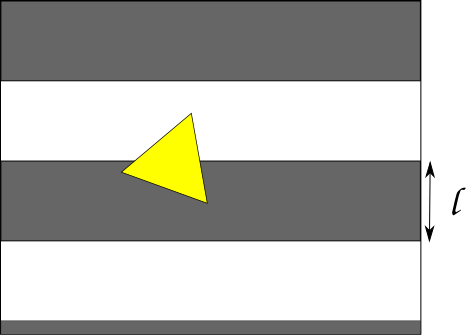
\includegraphics[scale=0.5]{path6509.png}
\caption{\label{color} Find a title}
\end{figure}

%CLASSE DE SOLUTIONS?

\subsection{3 colours}

 With three colors, we use the Moser spindle - that has at least one of its $11$ edges with both ends of the same colour.
 We similarly use lemma ~\ref{huitre} to get that in the case of three colours,
 the probability that both endpoints have the same colour is at least $\frac{1}{11}$ with the first needle throwing process. 

We don't know if the previous bound is optimal, however we have found the
following colouring which approaches this bound.
  

\subsection{Other extensions}

We can generalize the two processes in higher dimensions, and prove the
process equivalence. %A PRECISER

We remark that in higher dimension, the bounds possibly change : for
example, in 3 dimensions, the regular tetrahedron witnesses a better lower bound
of $\frac 1 6 >\frac 1 {11}$   

\section{Finite table}

\begin{figure}[h]
\center
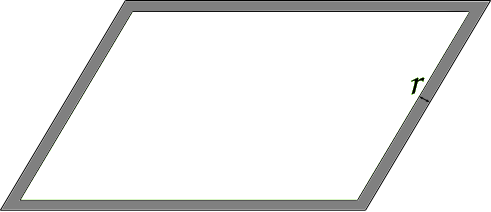
\includegraphics[scale=0.5]{tablefinie.png}
\caption{\label{tablefinie} Find a title}
%\flushleft
\end{figure}
The previous process can be modified to match a somewhat more practical view. In this section, we consider the process of needle throwing in a finite table. 
Formally, it is defined as follows :
\begin{process}
Denote by P a parallelogram (representing the table). 
\begin{itemize}
\item Choose a point uniformly in P for the lower point of the needle
\item Choose an angle theta uniformly in $[0 ; \Pi]$ such that the second end of the needle does not fall out of the table
\end{itemize}
\end{process}

Similarly to what was done in the previous section, we define a second process, consisting in throwing a triangle, and then choosing a edge on this triangle.
This will provide a bound on the probability for two colours.

\begin{process}
We therefore define an other needle choosing process :
\begin{itemize}
  \item let $\theta '$ (the orientation of our triangle) be chosen uniformly in $[0;\pi / 3]$ ;
  \item let $A'$ (the lowest vertex of the triangle) be a point in $P$ such that $A' + e^{i\theta '}$ is also in $P$, chosen uniformly among the points having this property ;
  \item let $B' = A' + e^{i \theta '}$ and $C' = A' + e^{i (\theta ' + \pi / 3 ) }$ ;
  \item let $(A'_1,A'_2)$ (lowest and highest endpoints of the needle) be a couple of points chosen uniformly between $(A',B')$, $(A',C')$, $(B',C')$.
\end{itemize}
Finally, let $p'$ be the probability that $A'_1$ and $A'_2$ have the same colour.
\end{process}


The result is the following :
\begin{lemma}
Denote by $p$ the probability that both ends have the same colour when throwing the needle on a finite table, then :
 $$ | p - p'| \leq \frac{\mathcal{P}}{\mathcal{A}} $$

In particular, this bound is sharp when the dimensions of the table goes to infinity. It follows immediately from this that : $p \geq \frac13 + \frac{\mathcal{P}}{\mathcal{A}}$ \\
The proof can be adapted to circular tables, or more generally to any table whose shape is not too complicated. \\
(*Say something about wether it can be adapted or not to moser*)
\end{lemma}


%\iffalse
%\subsection*{First proof}
%
%\begin{lemma}
% Let $p$ be the probability that both $A_1$ and $A_2$ have same colour. Let $\mathcal{A}(P)$ (resp. $\mathcal{P}(P)$) be the area (resp. perimeter) of $P$. We have :
% \[p \geq \frac{1}{3} - \frac{\mathcal{P}(P)}{\mathcal{A}(P)} \]
%\end{lemma}
%
%\begin{proof}
%The main idea is that an equilateral triangle must have at least one edge having both endpoints of the same colour.
%It also gives essentially the same results to choose an equilateral triangle randomly, and then to choose on of its edges as our needle.
%
%
%\begin{process}
%We therefore define a second needle choosing process :
%\begin{itemize}
%  \item let $\theta '$ (the orientation of our triangle) be chosen uniformly in $[0;\pi / 3]$ ;
%  \item let $A'$ (the lowest vertex of the triangle) be a point in $P$ such that $A' + e^{i\theta '}$ is also in $P$, chosen uniformly among the points having this property ;
%  \item let $B' = A' + e^{i \theta '}$ and $C' = A' + e^{i (\theta ' + \pi / 3 ) }$ ;
%  \item let $(A'_1,A'_2)$ (lowest and highest endpoints of the needle) be a couple of points chosen uniformly between $(A',B')$, $(A',C')$, $(B',C')$.
%\end{itemize}
%and $p'$ as the probability that $A'_1$ and $A'_2$ have the same colour.
%\end{process}
%
%Clearly, because there are at least two vertex of a triangle with the same color, we have the inequality $$p' \geq \frac{1}{3} $$.
%
%To conclude the proof, it suffices to prove that $|p' - p| \leq \frac{\mathcal{P}(P)}{\mathcal{A}(P)}$.
%If we denote $U_0$ (resp. $U_1$) the set of points $M$ such that $c(M) = 0$ (resp. $1$), we have :
%\begin{eqnarray*}
%|p' - p| 
%  &=& | \mathbb{P}(A'_1 , A'_2 \in U_0) - \mathbb{P}(A_1 , A_2 \in U_0) + \mathbb{P}(A'_1 , A'_2 \in U_1) - \mathbb{P}(A_1 , A_2 \in U_1) | \\
%  &\leq& | \mathbb{P}(A'_1 , A'_2 \in U_0) - \mathbb{P}(A_1 , A_2 \in U_0) | + | \mathbb{P}(A'_1 , A'_2 \in U_1) - \mathbb{P}(A_1 , A_2 \in U_1) |
%\end{eqnarray*}
%
%Let's focus on the first term. 
%Decompose the first probability in three terms corresponding to the final choice of $(A',B')$, $(A',C')$ or $(B',C')$, and the second one in three terms according to the position of $\theta$ :
%\begin{eqnarray*}
%& & | \mathbb{P}(A'_1 , A'_2 \in U_0) - \mathbb{P}(A_1 , A_2 \in U_0) | \\
%&\leq& \frac{1}{3} | \mathbb{P}(A' \in U_0 , A' + e^{i \theta '} \in U_0) - \mathbb{P}(A_1 \in U_0 , A' + e^{i \theta} \in U_0 \ |\  \theta < \frac{\pi}{3} ) | \\
%&+& \frac{1}{3} | \mathbb{P}(A' \in U_0 , A' + e^{i(\theta ' + \pi / 3 ) } \in U_0) - \mathbb{P}(A_1 \in U_0 , A' + e^{i \theta} \in U_0 \ |\  \frac{\pi}{3} \leq \theta < \frac{2 \pi}{3} ) | \\
%&+& \frac{1}{3} | \mathbb{P}(A' + e^{i \theta '} \in U_0 , A' + e^{i(\theta ' + \pi / 3 ) } \in U_0) - \mathbb{P}(A_1 \in U_0 , A' + e^{i \theta} \in U_0 \ | \  \frac{2 \pi}{3} < \theta ) |
%\end{eqnarray*}
%
%Once again, let's focus on the first term. Let $\mathcal{P'}$ be the parallelogram  composed of the points of  $\mathcal{P}$ at a distance of at least one from the borders. Conditioning to the fact that the points $A$ and $A'$ fall on $\mathcal{P'}$, the two points are uniformly distributed in $\mathcal{P'}$, and independent of $\theta$ and $\theta'$. Thus this term is overestimated by the probability for $A$ and $A'$ to fall near the borders of the parallelogram. This probability is smaller than : $\mathcal{P}/\mathcal{A}$.
%
%\end{proof}
%
%
%\subsection*{Second proof}
%\fi


\end{document}
